% Compile with: pdflatex "One-Period Model and AD-AS.tex" (twice).
% Standalone source: all diagrams are drawn in TikZ; no external assets.
% Sources: IMG_1449-1451 = household (own notes); IMG_1432-1438 = firm/government;
% IMG_1429-1431 = AD extensions and money; IMG_1439-1448 = AS and AD-AS diagrams.
\documentclass[11pt,letterpaper]{article}
\usepackage[T1]{fontenc}
\usepackage{lmodern}
\usepackage[margin=0.85in]{geometry}
\usepackage{amsmath,amssymb,enumitem,parskip,needspace}
\usepackage{tikz}
\usetikzlibrary{arrows.meta}
\usepackage[hidelinks]{hyperref}
\hypersetup{pdftitle={A One-Period Model: From Household Choice to AD--AS},
  pdfsubject={Consolidated macroeconomics lecture notes}}
\setlength{\parindent}{0pt}
\setlength{\parskip}{6pt plus 1pt}
\setlength{\abovedisplayskip}{8pt plus 2pt minus 2pt}
\setlength{\belowdisplayskip}{8pt plus 2pt minus 2pt}
\setlength{\emergencystretch}{1.5em}
\setlist[itemize]{leftmargin=1.3em,itemsep=3pt,topsep=3pt,parsep=0pt}
\setlist[enumerate]{leftmargin=1.6em,itemsep=4pt,topsep=3pt,parsep=0pt}
\newcommand{\topic}[1]{\par\Needspace{4\baselineskip}\medskip\textbf{#1}\par\nobreak}
\newcommand{\w}{\omega}
\newcommand{\mpl}{\operatorname{MPL}}
\newcommand{\mpk}{\operatorname{MPK}}
\tikzset{axis/.style={-{Stealth[length=4pt,width=3pt]},line width=.55pt},
  curve/.style={line width=.85pt}, guide/.style={dashed,black!45,line width=.45pt},
  dot/.style={circle,fill,inner sep=1.5pt}, every node/.style={font=\small,text=black}}
\raggedbottom

\begin{document}
\begin{center}
  {\small\scshape Macroeconomic Theory --- Lecture Notes}\\[5pt]
  {\LARGE\bfseries A One-Period Model}\\[4pt]
  {\large From household choice to aggregate demand and supply}
\end{center}
\vspace{2pt}\hrule\vspace{5pt}

\textbf{The lecture's argument.} Households choose consumption and work; firms
choose employment; their interaction determines real output. With flexible wages,
rescaling nominal prices leaves this real allocation unchanged. With preset nominal
wages, demand changes can move employment and output temporarily. Money, investment
and trade enter later as extensions of the basic model.

\section{The household: consumption versus leisure}
Time is normalized to one. Let $c$ be consumption, $\ell$ hours worked and
$s=1-\ell$ leisure. The household receives nominal wages $W$, dividends $\Pi$
and pays lump-sum taxes $T$. The goods price is $P>0$. Define
\[
  \w\equiv\frac{W}{P}>0 \quad\text{(real wage)},\qquad
  b\equiv\frac{\Pi-T}{P}\quad\text{(real net non-wage income)}.
\]
$\Pi$ denotes profits (dividends); $\pi$ will denote inflation. The preference
parameter $\delta>0$ is the weight on leisure.

\topic{Problem and first-order conditions}
\begin{equation}
  \max_{c>0,\,0\leq\ell<1}\{\ln c+\delta\ln(1-\ell)\}
  \quad\text{s.t.}\quad Pc=W\ell+\Pi-T.
  \label{eq:household}
\end{equation}
Treat $W,P,\Pi,T$ as given when choosing $c$ and $\ell$. For an interior optimum,
\[
  \mathcal L=\ln c+\delta\ln(1-\ell)
       +\lambda(W\ell+\Pi-T-Pc).
\]
\begin{equation}
  \frac{1}{c}=\lambda P,\qquad
  \frac{\delta}{1-\ell}=\lambda W
  \quad\Longrightarrow\quad
  \boxed{\frac{\delta c}{1-\ell}=\w.}
  \label{eq:mrs}
\end{equation}
Read it as $\delta/(1-\ell)=\w\cdot(1/c)$:
\[
 \underbrace{\frac{\delta}{1-\ell}}_{\substack{\text{marginal cost of working}\\=\text{MU of leisure}}}
 \;=\;
 \underbrace{\w}_{\text{extra }c}\times\underbrace{\frac1c}_{\text{MU of }c}
 \quad\text{(marginal benefit of working)}.
\]

\topic{Solve for consumption and labour supply}
Substitute $c=\w\ell+b$ into \eqref{eq:mrs}:
\[
  \delta(\w\ell+b)=\w(1-\ell)
  \quad\Longrightarrow\quad (1+\delta)\w\ell=\w-\delta b.
\]
\begin{equation}
 \boxed{\quad
 c^*=\frac{\w+b}{1+\delta},\qquad
 \ell^*=\frac{1-\delta b/\w}{1+\delta},\qquad
 s^*=\frac{\delta}{1+\delta}\left(1+\frac{b}{\w}\right).
 \quad}
 \label{eq:choices}
\end{equation}
(Note the denominator is $1+\delta$, not $1-\delta$.) These formulas assume
$-\w<b<\w/\delta$; if $b\geq\w/\delta$ the household does not work ($\ell=0$, $c=b$).

\newpage
\section{Income effects, substitution effects and prices}
\topic{Higher non-wage income: hold the real wage fixed}
For the interior solution,
\[
 \frac{\partial c^*}{\partial b}=\frac{1}{1+\delta}>0,\qquad
 \frac{\partial s^*}{\partial b}=\frac{\delta}{(1+\delta)\w}>0,\qquad
 \frac{\partial\ell^*}{\partial b}=-\frac{\delta}{(1+\delta)\w}<0.
\]
Consumption and leisure are normal goods: more dividends or lower lump-sum taxes
allow the household to consume more and work less.

\topic{Higher real wages: hold real non-wage income fixed}
\begin{itemize}
 \item \textbf{Substitution effect:} leisure becomes more expensive in forgone
 consumption, so the household substitutes toward work.
 \item \textbf{Income effect:} greater earning power makes the household wealthier,
 increasing its demand for leisure and reducing work.
\end{itemize}
The net effect in this particular log-utility model is
\begin{equation}
 \frac{\partial\ell^*}{\partial\w}
   =\frac{\delta b}{(1+\delta)\w^2}
   \begin{cases}>0,&b>0,\\=0,&b=0,\\<0,&b<0.\end{cases}
 \label{eq:supplysign}
\end{equation}
The lecture draws labour supply sloping upward, i.e.\ the substitution effect
dominates. In this log-utility model that holds exactly when $b>0$ (at $b=0$
the two effects cancel). In equilibrium $b=(\Pi-T)/P=(\alpha-g)Y$ (Section 3),
so the condition is $\alpha>g$: capital's share exceeds the government's spending share.

\begin{center}
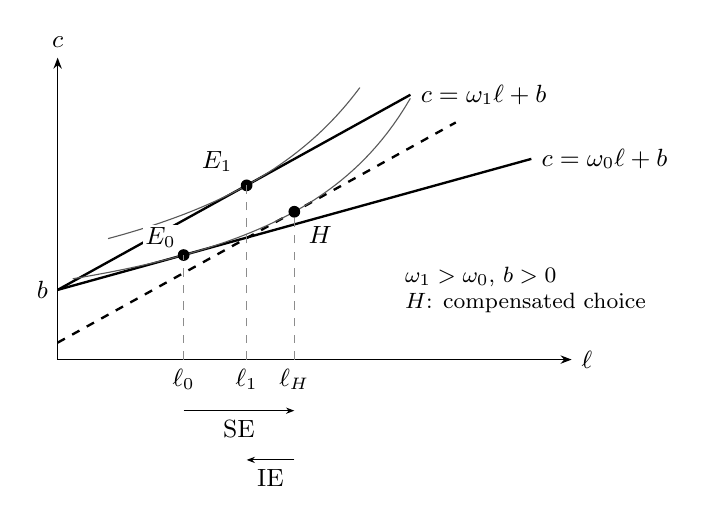
\begin{tikzpicture}[x=6.4cm,y=1.18cm]
 \draw[axis] (0,0) -- (1.02,0) node[right] {$\ell$};
 \draw[axis] (0,0) -- (0,3.25) node[above] {$c$};
 \draw[curve] (0,.75) -- (.94,2.16) node[right] {$c=\w_0\ell+b$};
 \draw[curve] (0,.75) -- (.70,2.85) node[right] {$c=\w_1\ell+b$};
 \draw[curve,dashed] (0,.18198) -- (.79,2.55198);
 \draw[black!65,domain=.03:.70,samples=60] plot (\x,{.84375/(1-\x)});
 \draw[black!65,domain=.10:.60,samples=60] plot (\x,{1.171875/(1-\x)});
 \node[left] at (0,.75) {$b$};
 \node[dot,label={[fill=white,inner sep=1pt]above left:$E_0$}] at (.25,1.125) {};
 \node[dot,label={above left:$E_1$}] at (.375,1.875) {};
 \node[dot,label={below right:$H$}] at (.46967,1.59099) {};
 \draw[guide] (.25,0) -- (.25,1.125);
 \draw[guide] (.375,0) -- (.375,1.875);
 \draw[guide] (.46967,0) -- (.46967,1.59099);
 \node[below] at (.25,0) {$\ell_0$};
 \node[below] at (.375,0) {$\ell_1$};
 \node[below] at (.46967,0) {$\ell_H$};
 \draw[-{Stealth[length=3pt]}] (.25,-.55) -- (.46967,-.55)
   node[midway,below] {SE};
 \draw[-{Stealth[length=3pt]}] (.46967,-1.08) -- (.375,-1.08)
   node[midway,below] {IE};
 \node[align=left,anchor=west,font=\footnotesize] at (.67,.75)
   {$\w_1>\w_0$, $b>0$\\$H$: compensated choice};
\end{tikzpicture}
\end{center}
\vspace{-7pt}
{\small The budget line in $(\ell,c)$ space has slope $\w$ and intercept $b$.
$E_0\to H$ holds utility fixed (substitution effect, SE); $H\to E_1$ is the income
effect (IE). Indifference curves slope upward because work ($\ell$) is a ``bad''.}

\topic{Inflation: neutral if indexed, costly if income is sticky}
If $P,W,\Pi,T$ all rise in the same proportion (nominal income is
\emph{indexed} to inflation), $\w$ and $b$ do not change, so neither do
$c^*,\ell^*,s^*$: inflation is \emph{neutral}.
If instead nominal income is slow to adjust (economists argue \emph{wages are
sticky}), a rise in $P$ erodes purchasing power. With $W,\Pi,T$ fixed,
\[
 c^*=\frac{W+\Pi-T}{(1+\delta)P}\downarrow,\qquad
 \ell^*=\frac{1-\delta(\Pi-T)/W}{1+\delta}\ \text{is unchanged}.
\]

\newpage
\section{Firms, government and the real equilibrium}
\topic{The firm's problem}
Capital $K>0$ is fixed for the period; $A>0$ is labour-augmenting productivity.
With $0<\alpha<1$, the competitive firm chooses employment $L$:
\begin{equation}
 \max_{L\geq0}\{\Pi=PY-WL\},\qquad
 Y=(AL)^{1-\alpha}K^\alpha.
 \label{eq:firm}
\end{equation}
The first-order condition equates the value of an extra worker's output to its cost:
\begin{equation}
 P\underbrace{(1-\alpha)A^{1-\alpha}L^{-\alpha}K^\alpha}_{\mpl}
   =W
 \quad\Longleftrightarrow\quad
 \w=\mpl=(1-\alpha)\frac{Y}{L}.
 \label{eq:mpl}
\end{equation}
Hence labour demand is
\begin{equation}
 \boxed{L^d(\w)=\left[\frac{(1-\alpha)A^{1-\alpha}K^\alpha}{\w}\right]^{1/\alpha}.}
 \label{eq:ld}
\end{equation}
It slopes downward because labour has diminishing marginal product when capital
is fixed. Higher $A$ or $K$ raises labour demand at any given real wage.

\topic{Income shares and dividends}
Multiplying \eqref{eq:mpl} by $L$ gives
\begin{equation}
 WL=(1-\alpha)PY,\qquad
 \Pi=PY-WL=\alpha PY,\qquad \frac{\Pi}{P}=\alpha Y=\mpk K.
 \label{eq:shares}
\end{equation}
The firm owns the capital, so the payment to capital, $\mpk\cdot K$, takes the
form of profit or dividend payments to households. Note that dividends are
\emph{indexed for inflation}: for given real output they rise in proportion to $P$.

\topic{Government and goods-market clearing}
Let $g$ ($0\leq g<1$) be the government's propensity to spend, and assume a
balanced budget:
\begin{equation}
 PG=g\,PY,\qquad T=PG=g\,PY.
 \label{eq:government}
\end{equation}
Taxes rise with the nominal tax base $PY$, so they too are indexed for inflation.
(The household still treats $T$ as lump sum.)

\textbf{Consequence.} Both $\Pi$ and $T$ scale with $P$, so real non-wage income
\[
 b=\frac{\Pi-T}{P}=(\alpha-g)Y
\]
does not depend on $P$. Only the nominal wage $W$ can fail to keep up with prices,
which is why the AS analysis below focuses on sticky wages.

With one representative household, $L=\ell$ and $C=c$. Combining its budget with
$\Pi=PY-WL$ gives
\[
 PC=PY-T\quad\Longrightarrow\quad C+G=Y,\qquad C=(1-g)Y.
\]
There is no saving, investment or trade in this one-period benchmark.

\topic{Completing the benchmark: what determines potential output?}
Combine the household's condition \eqref{eq:mrs}, $C=(1-g)Y$ and \eqref{eq:mpl}:
\[
 \frac{\delta(1-g)Y}{1-L}=\frac{(1-\alpha)Y}{L}
 \quad\Longrightarrow\quad
 \boxed{L^n=\frac{1-\alpha}{1-\alpha+\delta(1-g)},\qquad
 Y^n=(AL^n)^{1-\alpha}K^\alpha.}
\]
(This step is not on the slides, but it closes the model.) Neither expression
contains $P$: real fundamentals alone pin down potential output $Y^n$. On the
board this is $Y_0=(AL_0)^{1-\alpha}K^\alpha$.

\newpage
\section{Aggregate demand and the monetary extension}
\topic{What the household problem gives us}
From the household problem we get two curves (board sketches):
\begin{itemize}
 \item a \textbf{downward-sloping AD curve} in $(Y,P)$: with nominal income slow
 to adjust, $c^*=(W+\Pi-T)/[(1+\delta)P]$ falls as $P$ rises;
 \item an \textbf{upward-sloping labour-supply curve} $\ell(\w)$ (when $b>0$; Section 2).
\end{itemize}

\topic{Add investment and international trade (informally)}
The model is too simple: it has no dynamics (no intertemporal decisions, so no
saving and investment) and no international trade. We could add these formally;
for now, add them to AD informally:
\begin{equation}
 \mathrm{AD}=C+G\quad\Longrightarrow\quad \mathrm{AD}=C+I+G+NX.
 \label{eq:ad}
\end{equation}
In addition to $P$, assume:
\begin{itemize}
 \item \textbf{Interest rate:} $C$ and $I$ depend negatively on the interest rate $r$:
 $r\downarrow\Rightarrow C,I\uparrow\Rightarrow\mathrm{AD}$ shifts right.
 \item \textbf{Exchange rate:} $NX$ depends positively on the real exchange rate
 $er\cdot P^f/P$, where $er$ = Canadian dollars per unit of foreign currency and
 $P^f$ = foreign price level. Hence $NX$ depends \emph{negatively} on $P$ too,
 another reason AD slopes down.
\end{itemize}

\topic{Money: cash-in-advance, inflation tax and seigniorage}
In more complicated models, money is needed for consumption expenditure
(\textbf{cash-in-advance}, CIA, models). Then a price increase lowers real money
holdings $M/P$ and so reduces purchasing power.
\begin{itemize}
 \item \textbf{Inflation tax:} inflation acts like a tax on nominal balances, since
 it erodes their real value (roughly $\pi\cdot M/P$).
 \item \textbf{Seigniorage:} government revenue from money creation (real value
 $\Delta M/P$).
\end{itemize}
Suppose the government expands the money supply to pay for \emph{additional}
spending. This causes inflation, which lowers private agents' real balances, so
$c\downarrow$.

These are \emph{demand-side} effects of price changes, but there can also be a
\emph{supply-side} effect: to avoid the inflation tax, consumers may switch to
items that do not require money, i.e.\ leisure. Then $\ell\downarrow\Rightarrow Y\downarrow$.
\textbf{For now, ignore the effect of $M/P$ on the position of the labour-supply curve.}

\newpage
\section{Aggregate supply: flexible versus preset wages}
\topic{Flexible wages: vertical long-run aggregate supply}
Labour demand and supply determine a real wage $\w^n$ and employment $L^n$.
If $P$ rises while the nominal wage initially stays fixed, $W/P$ falls. But at
the lower real wage firms want more labour than households supply, and this
excess demand for labour pushes $W$ up. Once wages fully adjust,
\[
 \frac{W_1}{P_1}=\frac{W_0}{P_0}=\w^n,\qquad
 L=L^n,\qquad Y=Y^n.
\]
Thus LRAS is vertical at $Y^n$: a higher $P$ is matched by a higher $W$, with no
real effect. (``Long run'' here just means wages have adjusted.)

\begin{center}
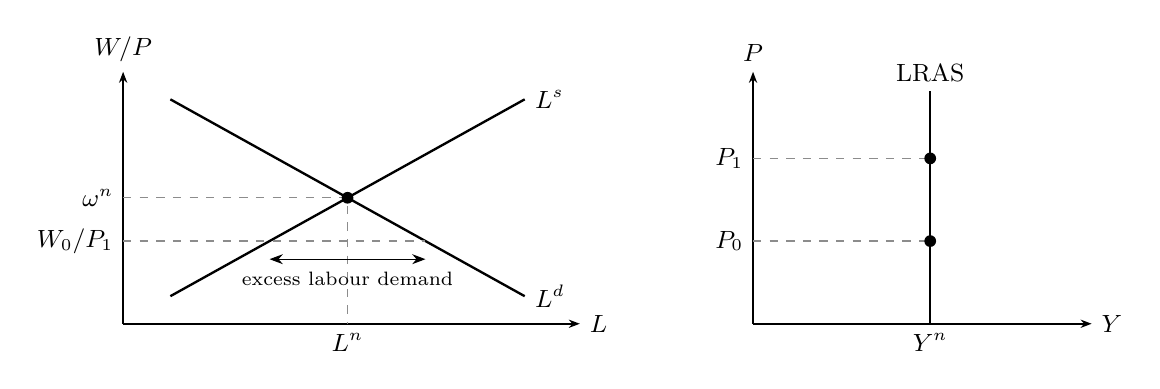
\begin{tikzpicture}[x=1cm,y=1cm]
 \begin{scope}
  \draw[axis] (0,0) -- (5.8,0) node[right] {$L$};
  \draw[axis] (0,0) -- (0,3.2) node[above] {$W/P$};
  \draw[curve] (.6,2.85) -- (5.1,.35) node[right] {$L^d$};
  \draw[curve] (.6,.35) -- (5.1,2.85) node[right] {$L^s$};
  \draw[guide] (0,1.6) node[left] {$\w^n$} -- (2.85,1.6) -- (2.85,0);
  \draw[guide] (0,1.05) node[left] {$W_0/P_1$} -- (3.84,1.05);
  \node[dot] at (2.85,1.6) {};
  \node[below] at (2.85,0) {$L^n$};
  \draw[<->,>=Stealth] (1.86,.82) -- (3.84,.82);
  \node[below,font=\scriptsize] at (2.85,.78) {excess labour demand};
 \end{scope}
 \begin{scope}[xshift=8cm]
  \draw[axis] (0,0) -- (4.3,0) node[right] {$Y$};
  \draw[axis] (0,0) -- (0,3.2) node[above] {$P$};
  \draw[curve] (2.25,0) -- (2.25,2.95) node[above] {LRAS};
  \draw[guide] (0,1.05) node[left] {$P_0$} -- (2.25,1.05);
  \draw[guide] (0,2.1) node[left] {$P_1$} -- (2.25,2.1);
  \node[dot] at (2.25,1.05) {};
  \node[dot] at (2.25,2.1) {};
  \node[below] at (2.25,0) {$Y^n$};
 \end{scope}
\end{tikzpicture}
\end{center}
{\small A temporary fall in the real wage creates excess labour demand; after
$W$ adjusts, employment and output return to $L^n$ and $Y^n$.}

\topic{Preset nominal wages: upward-sloping short-run aggregate supply}
If $W=\bar W$ is fixed by a short-term contract, a higher $P$ lowers the real
cost of labour. Firms want to hire more and produce more:
\[
 P\uparrow\quad\Longrightarrow\quad \bar W/P\downarrow
 \quad\Longrightarrow\quad L^d\uparrow\quad\Longrightarrow\quad Y\uparrow.
\]
Using \eqref{eq:ld} and the production function gives the firm's supply schedule:
\begin{equation}
 Y^s(P;\bar W)=A^{1-\alpha}K^\alpha
 \left[\frac{(1-\alpha)A^{1-\alpha}K^\alpha P}{\bar W}\right]^{(1-\alpha)/\alpha}.
 \label{eq:sras}
\end{equation}
It slopes upward in $(Y,P)$ space. A higher preset wage shifts SRAS up/left:
less output is profitable at any given price.

\textbf{Implicit assumption.} In the short run employment is set by labour
\emph{demand}: under the contract, workers supply the hours firms ask for at $\bar W$.
That is how employment can rise above $L^n$ even though the real wage has fallen
(households would not choose those hours freely at that wage).

\newpage
\section{A demand expansion: short run to long run}
Start at $a$, with $Y_0=Y^n$, price $P_0$ and nominal wage $W_0$. Suppose a lower
interest rate raises consumption and investment, shifting AD to the right.
Hold productivity, capital and the fiscal share fixed.

\begin{center}
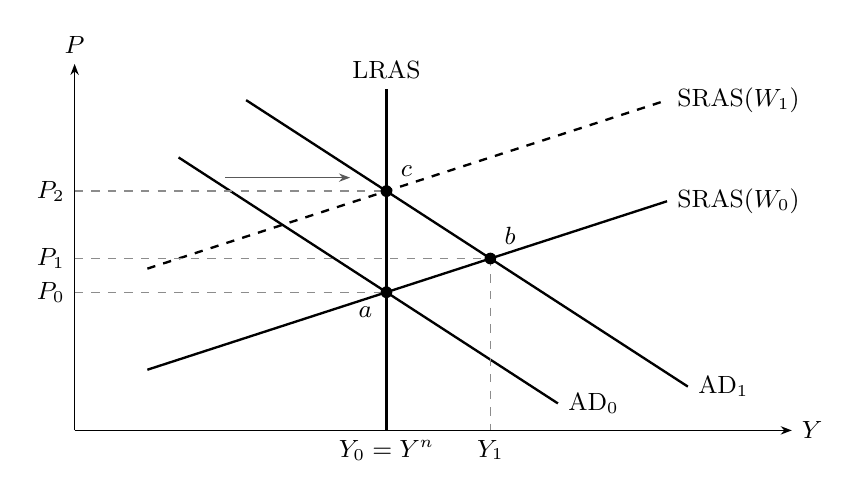
\begin{tikzpicture}[x=1.32cm,y=1.07cm]
 \draw[axis] (0,0) -- (6.9,0) node[right] {$Y$};
 \draw[axis] (0,0) -- (0,4.35) node[above] {$P$};
 \draw[curve] (3,0) -- (3,4.05) node[above] {LRAS};
 \draw[curve] (.7,.72) -- (5.7,2.72)
     node[right] {$\mathrm{SRAS}(W_0)$};
 \draw[curve,dashed] (.7,1.92) -- (5.7,3.92)
     node[right] {$\mathrm{SRAS}(W_1)$};
 \draw[curve] (1,3.24) -- (4.65,.32) node[right] {$\mathrm{AD}_0$};
 \draw[curve] (1.65,3.92) -- (5.9,.52) node[right] {$\mathrm{AD}_1$};
 \draw[guide] (0,1.64) node[left] {$P_0$} -- (3,1.64);
 \draw[guide] (0,2.04) node[left] {$P_1$} -- (4,2.04) -- (4,0);
 \draw[guide] (0,2.84) node[left] {$P_2$} -- (3,2.84);
 \node[dot,label={below left:$a$}] at (3,1.64) {};
 \node[dot,label={above right:$b$}] at (4,2.04) {};
 \node[dot,label={above right:$c$}] at (3,2.84) {};
 \node[below] at (3,0) {$Y_0=Y^n$};
 \node[below] at (4,0) {$Y_1$};
 \draw[-{Stealth[length=4pt]},black!65] (1.45,3.0) -- (2.65,3.0);
\end{tikzpicture}
\end{center}
\vspace{-6pt}
\begin{enumerate}
 \item \textbf{Short run: $a\to b$.} $W_0$ is preset. Prices rise to $P_1$,
 the real wage falls, and firms expand employment to $L_1>L^n$. Output rises
 to $Y_1>Y^n$ along the initial SRAS curve.
 \item \textbf{Wage adjustment: $b\to c$.} Contracts reset and nominal wages
 rise to $W_1$. SRAS shifts up/left until output returns to $Y^n$.
 The final price is $P_2>P_1>P_0$, with $W_1/P_2=W_0/P_0$.
\end{enumerate}
The demand expansion has a temporary real effect (output) and a permanent
nominal effect (higher price level).

\topic{The final equation: unexpected inflation and output}
The lecture ends with the summary supply relation
\begin{equation}
 \boxed{Y=Y^n+a(\pi-\pi^e)+e,\qquad a>0.}
 \label{eq:surprise}
\end{equation}
$\pi^e$ is the inflation workers expected when they set their wage contracts,
and $e$ is a supply shock (it shifts AS left or right).
\begin{itemize}
 \item The contract wage builds in expected inflation. If actual inflation is
 higher than expected ($\pi>\pi^e$), the real wage is eroded, firms hire more and
 $Y>Y^n$. This is the move $a\to b$ above.
 \item If inflation is correctly anticipated ($\pi=\pi^e$) and $e=0$, then
 $Y=Y^n$. This is point $c$: only surprises have real effects.
\end{itemize}
This is equation (2) of the next topic, \emph{Monetary Policy: Rules vs.\ Discretion} (there written with $Y_n$).

\end{document}
